\documentclass{beamer}
\usetheme{metropolis}

\usepackage{tcolorbox}
\tcbuselibrary{skins}

\newtcolorbox{mybubble}[1][]{
  enhanced jigsaw,
  borderline={1pt}{-2pt}{gray, sharp corners},
  frame hidden,
  left=1mm,
  right=1mm,
  fontupper=\scriptsize,
  arc=1mm,
  #1
}

\title{Exploring the Sentiment of Steam Reviews with Naive Bayes and Support Vector Machine}
\author{Puttisan "Ninja" Mukneam}
\institute{Pitzer College}
\date{\today}

% Customize footline
\setbeamertemplate{footline}
{
  \leavevmode%
  \hbox{%
  \begin{beamercolorbox}[wd=.25\paperwidth,ht=2.25ex,dp=1ex,center]{author in head/foot}%
    \usebeamerfont{author in head/foot}\insertauthor
  \end{beamercolorbox}%
  \begin{beamercolorbox}[wd=.75\paperwidth,ht=2.25ex,dp=1ex,center]{title in head/foot}%
  \end{beamercolorbox}}%
  \vskip0pt%
}

\begin{document}

\begin{frame}
\titlepage
\end{frame}

\section{Introduction}

\begin{frame}{NLP: Sentiment Analysis}

Sentiment analysis, also known as opinion mining, is a subfield of natural language processing (NLP) that focuses on extracting subjective information from text data. The primary goal of sentiment analysis is to determine the sentiment or emotional tone behind a series of words, which can be used to understand the attitudes, opinions, and emotions expressed by the author. Sentiment analysis is
widely applied in various domains, including social media monitoring, product reviews, customer, feedback analysis, and market research, among others.
    
\end{frame}

\begin{frame}{Steam}
\begin{itemize}
\item Steam platform: largest digital distribution platform for video games
\end{itemize}

\includegraphics[width = \textwidth]
{1.png}
\centering
\end{frame}

\begin{frame}{Steam Review}

\includegraphics[width = \textwidth]
{2.png}
\centering
\end{frame}

\begin{frame}{Steam Review Dataset [1]}
\begin{itemize}
\item Approximately 6.8 million reviews.
\end{itemize}
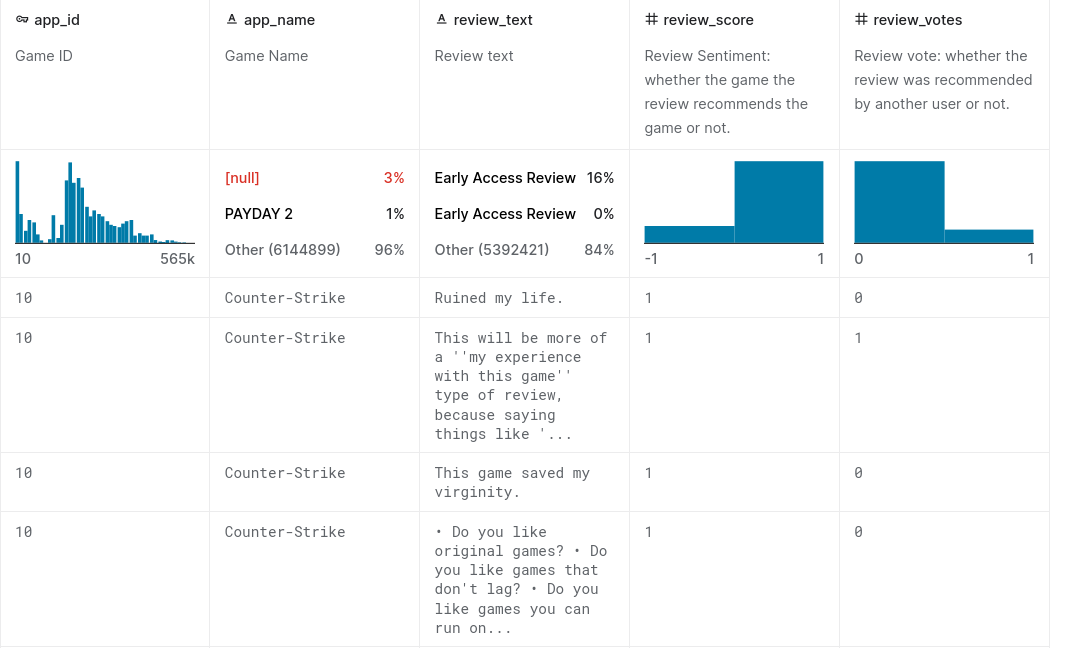
\includegraphics[width = \textwidth]
{fig_1.png}
\centering
\end{frame}

\section{Methods}
\begin{frame}{Data Collection and Preprocessing}
\begin{itemize}
\item First, 1M rows from the dataset.
\item Only interested in review\_text and review\_score column
\item Performed text preprocessing: Remove remove NAs, duplicates rows, traling space, special characters, stopwords.
\item Example: Before
\begin{mybubble}
"I hecking love Dota :3 (LoL is a terrible game btw.)"
\end{mybubble}
\item  After
\begin{mybubble}
    (w/ stopwords)"i hacking love dota lol is a terrible game btw"\\
    (w/o stopwords):"hecking love dota lol terrible game btw"
\end{mybubble}
\end{itemize}
\end{frame}

\begin{frame}{Text Vectorization: Bags of Words vs TFIDF}
\begin{itemize}
\item Importance weighting: Frequency, rarity, Importance
\item Reducing the impact of stopwords 
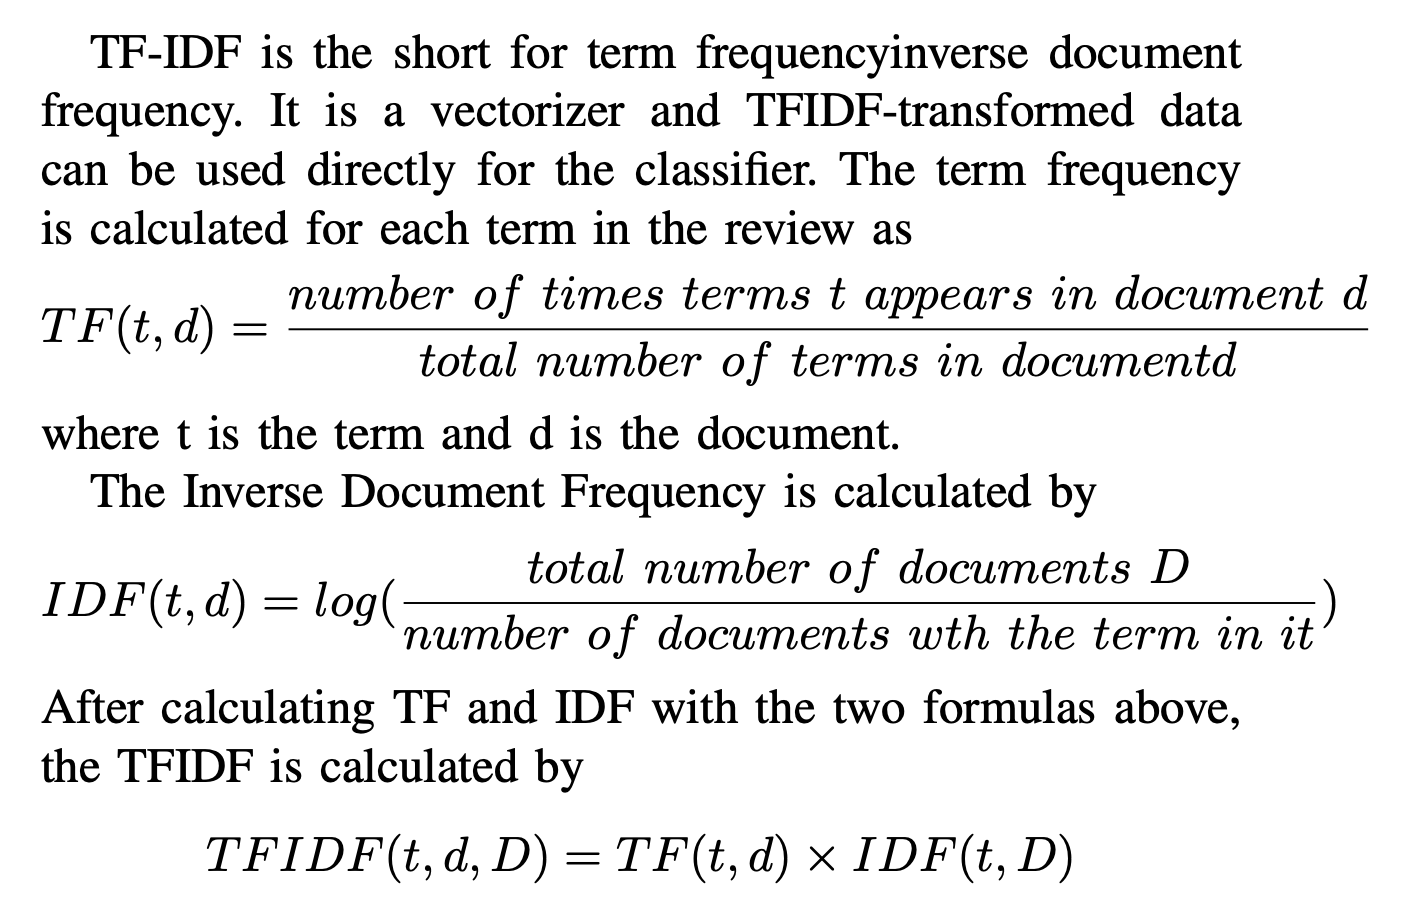
\includegraphics[width=\textwidth]{3.png}
\end{itemize}

\end{frame}

\begin{frame}{Multinomial Naive Bayes}
Given a document $d$ and a class label $c$, Bayes' theorem can be expressed as:

\begin{equation}
P(c|d) = \frac{P(d|c)P(c)}{P(d)}
\end{equation}

\begin{equation}
P(d|c)P(c) = P(w_1, w_2, \dots, w_n|c)P(c)
\end{equation}

where $w_1, w_2, \dots, w_n$ are the words in the document.

\end{frame}

\begin{frame}{Multinomial Naive Bayes continue}
\begin{equation}
P(w_1, w_2, \dots, w_n|c)P(c) = P(c)\prod_{i=1}^{n} P(w_i|c)
\end{equation}

To classify a document, we choose the class $c^*$ with the highest probability:

\begin{equation}
c^* = \arg\max_c P(c)\prod_{i=1}^{n} P(w_i|c)
\end{equation}
\end{frame}

\begin{frame}{Laplacian Smoothing}
    In practice, some words in the test data may not be present in the training data, leading to a zero probability for $P(w_i|c)$, which can cause issues in classification. To address this, Laplacian smoothing (also known as additive smoothing) is applied, which assigns a small non-zero probability to unseen words.

Given a word $w_i$ and a class $c$, the smoothed probability is calculated as:

\begin{equation}
P(w_i|c) = \frac{f_{w_i, c} + \alpha}{\sum_{w \in V} (f_{w, c} + \alpha)}
\end{equation}

where $f_{w_i, c}$ is the frequency of word $w_i$ in class $c$, $V$ is the vocabulary, and $\alpha$ is the smoothing parameter. A common choice for $\alpha$ is 1 (Laplace smoothing) or values between 0 and 1 (Lidstone smoothing).
\end{frame}
    

\begin{frame}{Linear SVM}
\textbf{Goal}: to find the optimal hyperplane that separates the data points of different classes with the maximum margin
\\
The decision function is a linear combination of the input features:

\begin{equation}
f(x) = w^T x + b
\end{equation}

where $w$ is the weight vector, $x$ is the input feature vector, and $b$ is the bias term.

The goal is to minimize the following objective function:

\begin{equation}
\frac{1}{2} |w|^2 + C \sum_{i=1}^{n} \xi_i
\end{equation}

subject to the some constrain function.
\end{frame}

\section{Results and Discussion}
\begin{frame}{Model Comparison MNB}

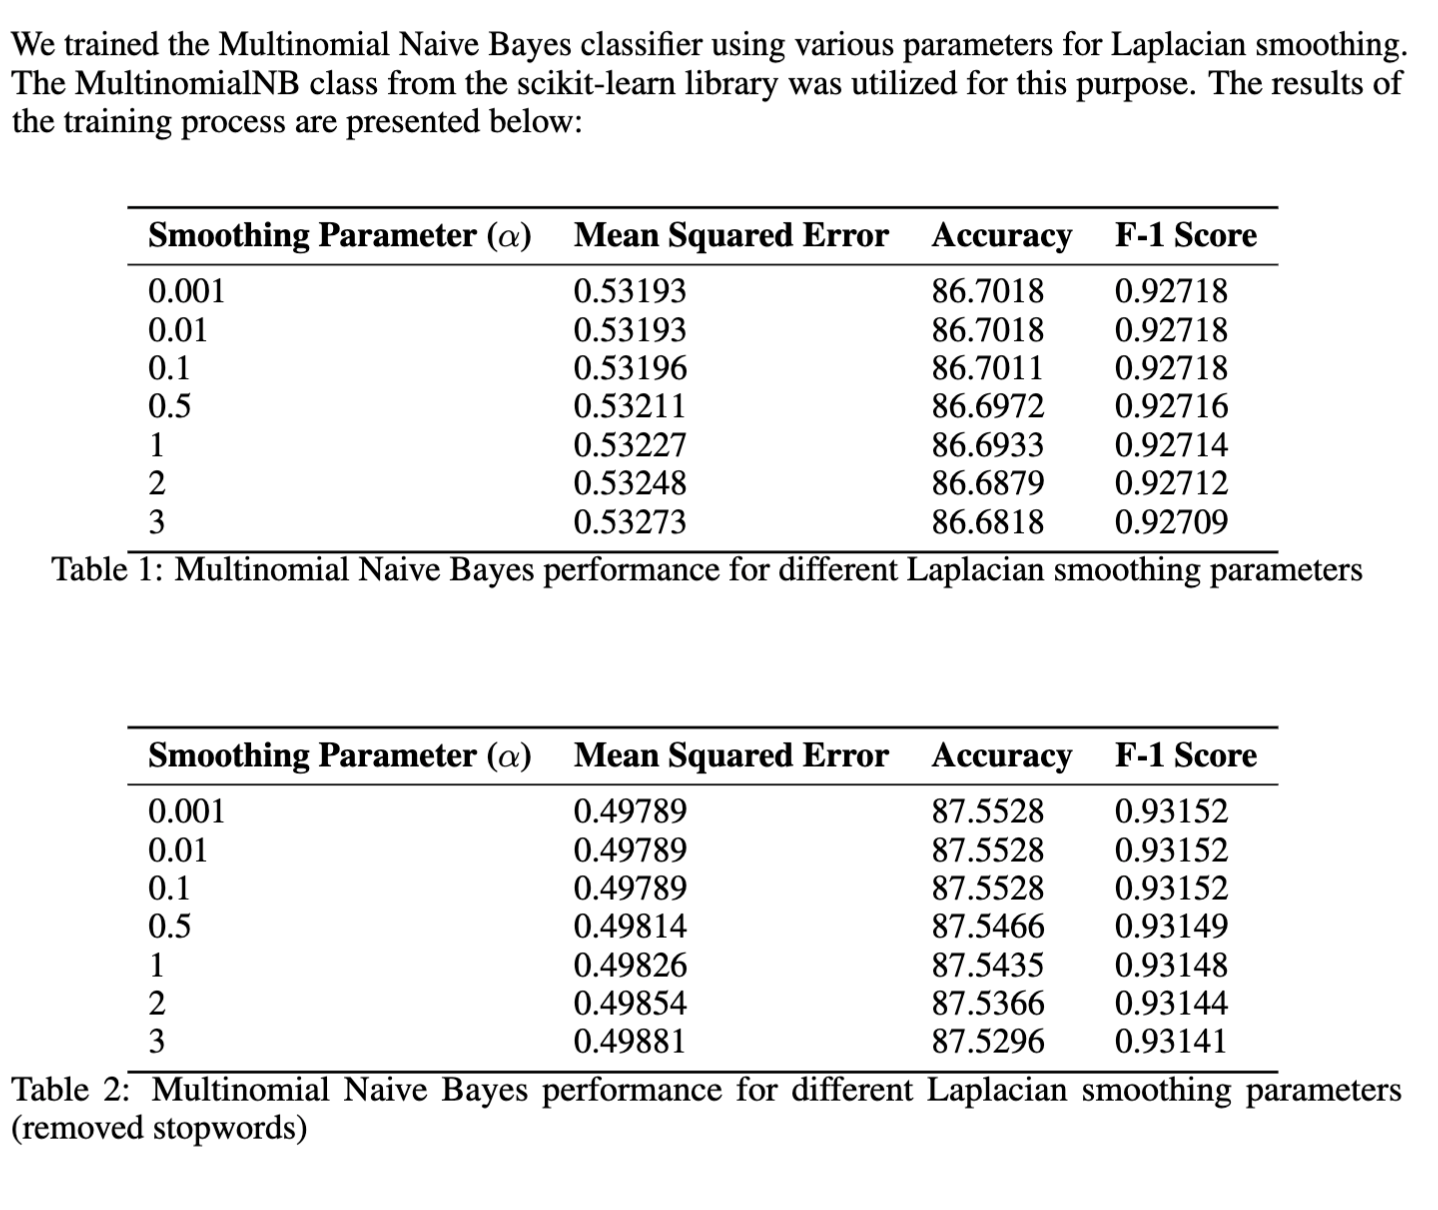
\includegraphics[width = 0.9\textwidth]{mb.png}



\end{frame}

\begin{frame}{Model Comparison SVM}

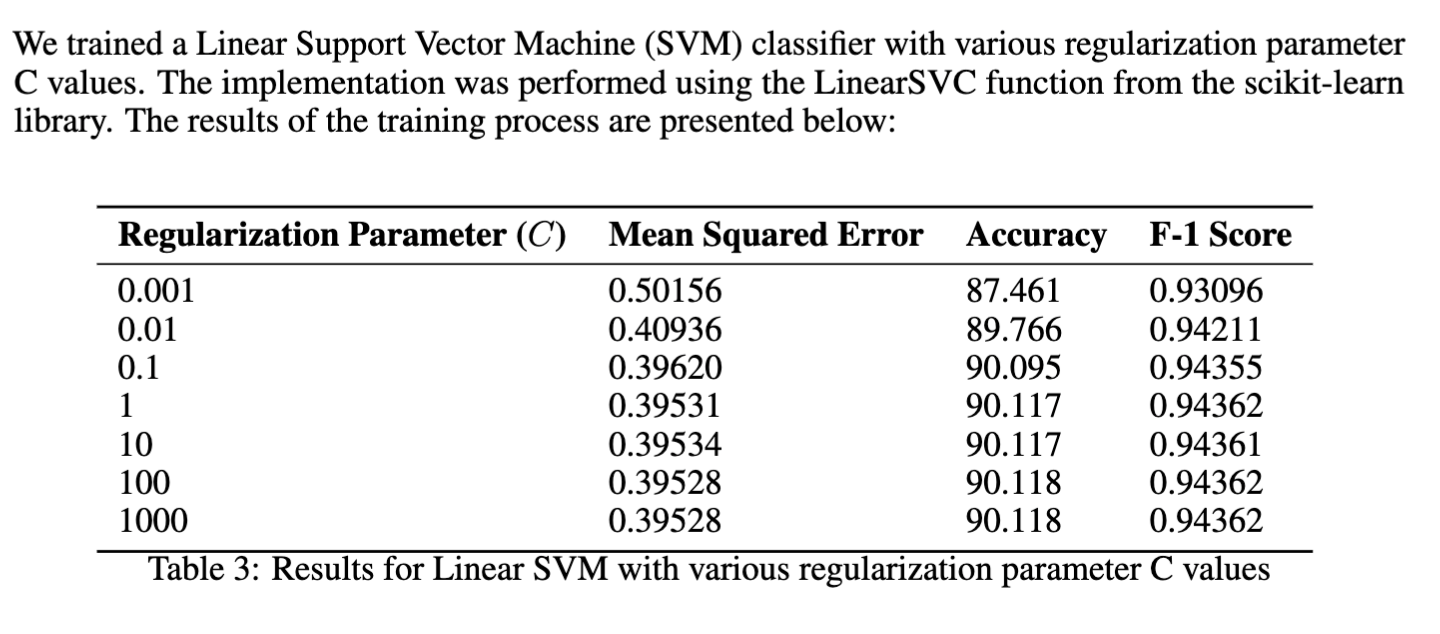
\includegraphics[width = 0.9\textwidth]{svm1.png}
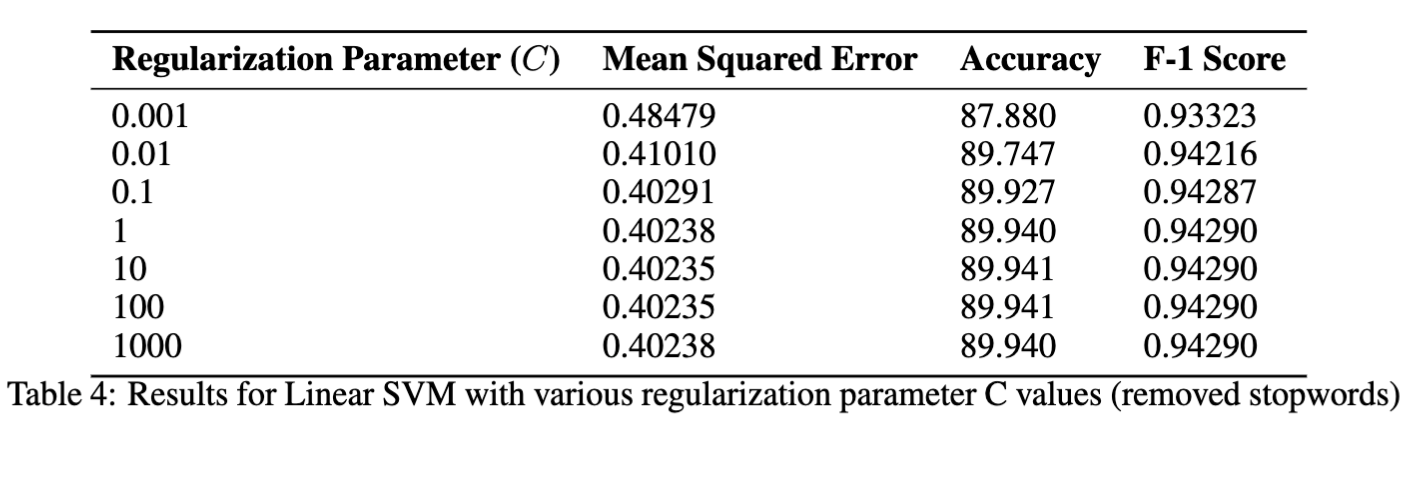
\includegraphics[width = 0.9\textwidth]{svm2.png}


\end{frame}

\begin{frame}{Testing}
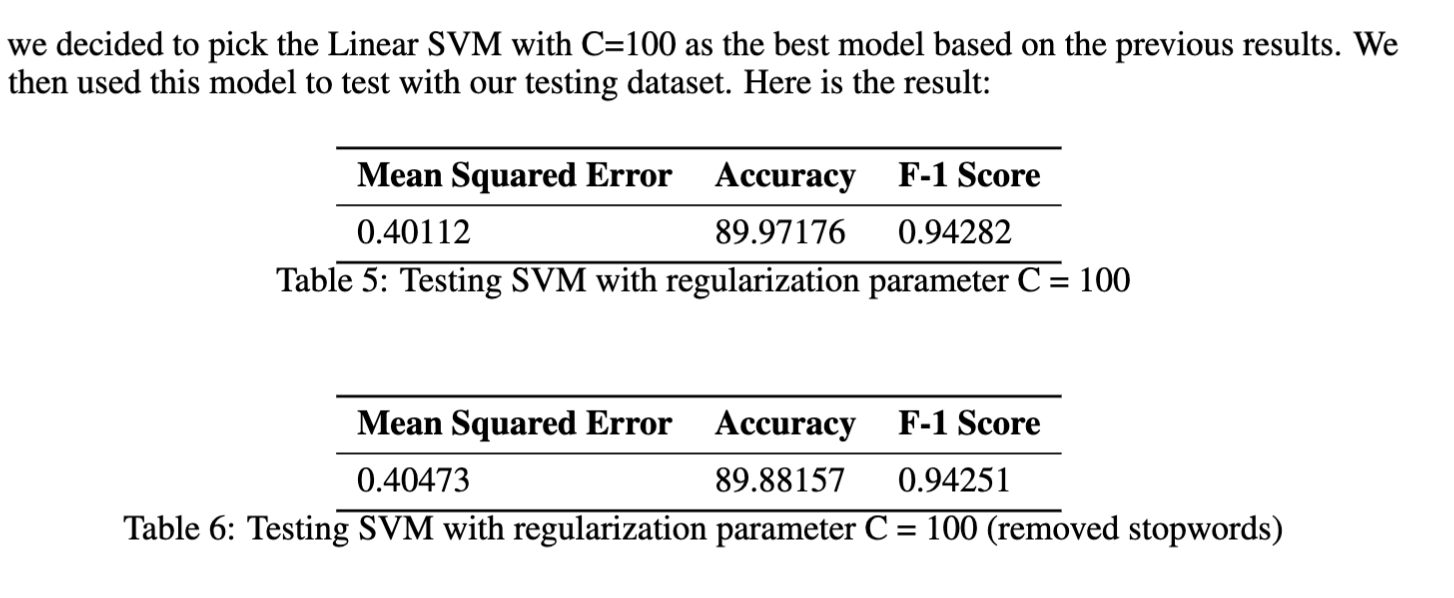
\includegraphics[width=0.9\textwidth]{testing.png}
    
\end{frame}

\begin{frame}{Future Work}
\begin{itemize}
    \item Deep Learning Algorithm: CNN, BERT, etc.
    \item Balancing the training and testing data set
    \item Try different SVM kernal
    \item Game Recommending system
    \item Hidden Markov Model
\end{itemize}
\end{frame}
\end{document}



